
%%%%%%%%%%%%%%%%%%%%%%%%%%%%%%%%%%%%%%%%%%%%%%%%%%%%%%%%%%%
%% Capítulo 2: Polinomios Ortoganles Clásicos            %%
%%%%%%%%%%%%%%%%%%%%%%%%%%%%%%%%%%%%%%%%%%%%%%%%%%%%%%%%%%%


En el capítulo \ref{chap:introduccionPO} hemos mostrado una amplia introducción a la ortogonalidad y presentado ejemplos concretos de polinomios ortogonales. En este capítulo presentaremos las familias concretas de polinomios ortogonales más importantes: los \textit{polinomios ortogonales clásicos}. Estos son los polinomios de Hermite, Laguerre, Jacobi y Bessel. Estas familias presentan la peculiaridad de ser las únicas que verifican ciertas propiedades, entre las que destaca la \textit{ecuación diferencial de Pearson}. Estos polinomios, entre otras disciplinas pueden ser encontrados en problemas de Sturm-Liouville cuando se utilizan ecuaciones diferenciales hipergeométricas.

\begin{figure}[h]
    \centering
    \begin{tabular}{ccc}
        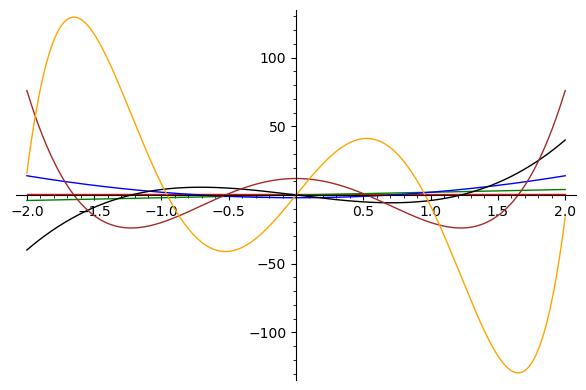
\includegraphics[width=5cm]{img/C2/hermite.png} & 
        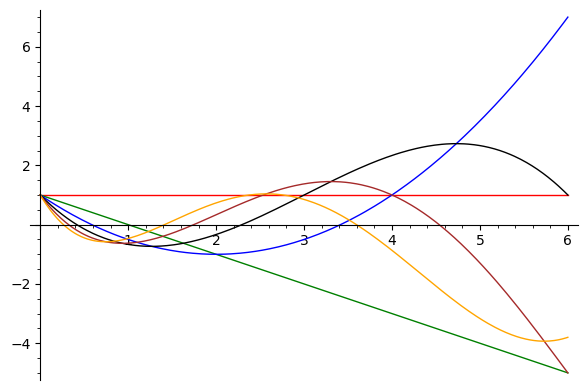
\includegraphics[width=5cm]{img/C2/laguerre.png} &
        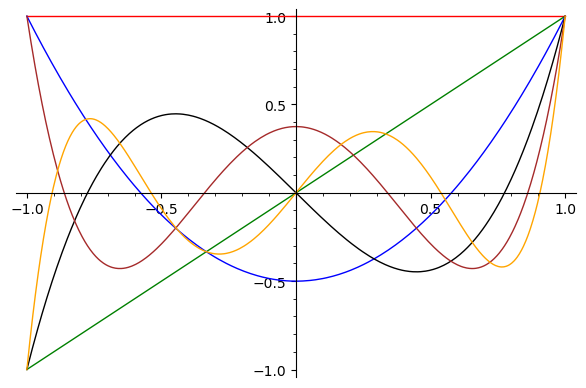
\includegraphics[width=5cm]{img/C2/jacobi.png} \\
        (a) Hermite $H_n$ & (b) Laguerre $L^{(0)}_n$ & (c) Jacobi $P^{(0,0)}_n$ 
    \end{tabular}
    \caption{Polinomios Ortogonales Clásicos}
    \label{img:graficas-clasicos}
\end{figure}

En las imágenes \ref{img:graficas-clasicos} podemos ver la representación gráfica, para parámetros concretos que definiremos próximamente, de los polinomios ortogonales de Hermite, Laguerre y Jacobi. Estas tres son las familias que mayor atención recibirán de nuestra parte al ser aquellas cuya ortogonalidad se manifiesta en intervalos reales.

\section{La ecuación de Pearson}

Para empezar, introduciremos una nueva notación para los funcionales de momentos que también se suele utilizar. Sea $\uu$ un funcional de momentos y $\{\mu_n\}$ su sucesión de momentos, entonces denotamos
\begin{equation}
    \label{eq:nueva-notacion-funcional}
    \begin{split}
        \uu:\mathbb P & \longrightarrow \R \\
        x^n & \longmapsto \left\langle \uu, x^n \right\rangle = \mu_n
    \end{split}
\end{equation}

A lo largo de este capítulo denotaremos como $\prodesc{\uu}{\pi(x)}$ a la aplicación del funcional $\uu$ a un polinomio $\pi(x)$.

Definimos a continuación dos operadores que actuán sobre los funcionales.

\begin{definicion}[Producto por un polinomio]
    Para cada polinomio $\pi$, definimos un nuevo funcional de momentos a partir de $\uu$ como
    \begin{equation}
        \begin{split}
            \pi\uu:\mathbb P & \longrightarrow \R \\
            \phi & \longmapsto \prodesc{\pi\uu}{\phi}=\prodesc{\uu}{\pi\phi}
        \end{split}
    \end{equation}
    
\end{definicion}

\begin{definicion}[Derivada]
    Definimos el funcional derivada como
    \begin{equation}
        \begin{split}
            D(\uu):\mathbb P & \longrightarrow \R \\
            \phi & \longmapsto \prodesc{D(\uu)}{\phi}=-\prodesc{\uu}{\phi'}
        \end{split}
    \end{equation}
    
\end{definicion}

A partir de estos dos operadores y esta nueva notación daremos una primera definición de lo que es una SPO clásica.

\begin{definicion}[SPO Clásica]
    La SPO $\{P_n  \}$ para el funcional $\uu$ se dice que es \textbf{clásica} (Hermite, Laguerre, Jacobi o Bessel) si existen polinomios $\sigma(x), \tau(x)$ con $\deg(\sigma)\leq 2$ y $\deg(\tau)= 1$ tales que el funcional $\uu$ verifica la ecuación diferencial
    \begin{equation}
        \label{eq:Pearson-u}
        D(\sigma \uu) = \tau \uu
    \end{equation}   
    La ecuación (\ref{eq:Pearson-u}) es conocida como la \textbf{ecuación de Pearson}.
\end{definicion}

En el caso de que la SPO sea ortogonal respecto a una función peso $\rho$, esto es, $\uu$ es de la forma
\begin{equation}
    \label{eq:funcional-peso}
    \prodesc{\uu}{\pi(x)} = \int_a^b \pi(x)\rho(x)dx,
\end{equation}
donde $(a,b)$ es cierto intervalo de la recta real donde $\rho > 0$, podemos deducir una condición equivalente.

\begin{lema}
    \label{lema:equivalencia-pearson}
    Sean $\rho(x)$ una función peso positiva en el intervalo $(a,b)$,$\uu$ el funcional definido como en (\ref{eq:funcional-peso}) y $\{P_n\}$ la SPO respecto a $\uu$. Si la función peso $\rho(x)$ es solución de la ecuación diferencial
    \begin{equation}
        \label{eq:Pearson-peso}
        [\sigma(x)\rho(x)]'=\tau(x)\rho(x)
    \end{equation}
    y además verifica las condiciones de frontera 
    \begin{equation}
        \label{eq:cond-frontera}
        \displaystyle\lim_{x\rightarrow a}\sigma(x)\rho(x)x^n = \displaystyle\lim_{x\rightarrow b}\sigma(x)\rho(x)x^n, \ \ \ n\geq 0,
    \end{equation}
    entonces la SPO $\{P_n\}$ es clásica, \textit{i.e.} $\uu$ verifica la ecuación de Pearson (\ref{eq:Pearson-u}).
    \cb{REVIEW Tengo que incluir en algún lugar que $\rho$ tiene momentos finitos, pero lo pongo aquí como una condición extra, lo incluyo en la definición de función peso, en el apartado de funcional de momentos...??}
\end{lema}
\begin{proof}
    Queremos comprobar la igualdad de funcionales $D(\sigma \uu)=\tau\uu$. Para ello, tengamos en cuenta que dos funcionales lineales son iguales si, y solo si actuán igual sobre una base de $\mathbb P$. Escogemos la base $\{x^n\}_{n\geq 0}$. Entonces tenemos que
    $$
    \prodesc{D(\sigma \uu)}{x^n} = -\prodesc{\sigma \uu}{n x^{n-1}}= -\prodesc{\uu}{\sigma(x)n x^{n-1}},
    $$
    aplicando (\ref{eq:funcional-peso}) e integración por partes, llegamos a
    \begin{equation*}
        \begin{split}
            \prodesc{D(\sigma \uu)}{x^n} &= -\int_a^b \sigma(x)n x^{n-1}\rho(x)dx = \left\{\begin{array}{ll}
                u = \sigma(x)\rho(x) & du=[\sigma(x)\rho(x)]'dx \\
                dv = n x^{n-1}dx & v = x^n
            \end{array}\right\} \\
            &= -\underbrace{\left[\sigma(x)\rho(x)x^n\right]_a^b}_{=0\text{ por (\ref{eq:cond-frontera})}}+ \int_a^b x^n [\sigma(x)\rho(x)]'dx\ \ \ \ \  \text{(aplicando (\ref{eq:Pearson-peso}))} \\
            &= \int_a^b x^n \tau(x)\rho(x)dx = \prodesc{\uu}{\tau(x)x^n} = \prodesc{\tau \uu}{x^n}
        \end{split}
    \end{equation*}
    
\end{proof}

\cb{REVIEW El recíproco tiene que ser cierto, pero no tengo la demostración }

\section{Deducción de las familias de polinomios ortogonales clásicos}
\label{section:deduccion-clasicos}

A partir del lema \ref{lema:equivalencia-pearson} podremos obtener las principales familias de polinomios ortogonales. Hemos impuesto que $\tau(x)=Ax+B$ sea un polinomio de grado exactamente $1$, por lo que tenemos cuatro grados de libertad a partir de las posibilidades de $\sigma(x)$, que supondremos mónico:

\begin{enumerate}
    \item \textbf{Caso I}: $\sigma(x) = 1$, $x\in\R$. En este caso obtendremos los llamados polinomios de Hermite.
    \item \textbf{Caso II}: $\sigma(x) = x-a$, $x\in[a,\infty)$. Haciendo el cambio de variable lineal $t=-(x-a)/A$ se tiene $\sigma(x) = x$ y $\tau(x)=-x+B$, $x\in[0,\infty)$. Con estos valores calcularemos los polinomios de Laguerre.
    \item \textbf{Caso III}: $\sigma(x) = (x-a)(b-x)$, $x\in[a,b]$. Con el cambio de variable $x = (b-a)/2t + (a+b)/2$ podemos escribir $\sigma(x)=1-x^2$ y $\tau=Ax+B$, $x\in[-1,1]$. Y así deduciremos los polinomios de Jacobi.
    \item \textbf{Caso IV}: $\sigma(x) = (x-a)^2$. En este último caso se obtienen los polinomios de Bessel. 
\end{enumerate}

\cb{REVIEW Pongo algún parrafito explicando por qué se eligen esos dominios?}

De acuerdo al lema \ref{lema:equivalencia-pearson}, si resolvemos la ecuación diferencial (\ref{eq:Pearson-peso}) asegurándonos de que las soluciones calculadas verifiquen las condiciones de frontera (\ref{eq:cond-frontera}), habremos hayado las funciones peso $\rho(x)$ para las cuales el funcional (\ref{eq:funcional-peso}) genera una SPO clásica. Nos centraremos principalmente en los casos I, II y III, en los cuales obtenemos un funcional definido positivo.

\subsection{Caso I: Polinomios de Hermite}
\label{subsection:Hermite}

Supongamos que $\sigma(x)=1$, $\forall x\in \R$. Tenemos entonces la ecuación diferencial
$$
\rho'(x) = (Ax+B) \rho(x), \ \ x\in\R.
$$
Esta ecuación es de variables separadas, por lo que podemos tomar
$$
    \int \dfrac{\rho'(x)}{\rho(x)}dx = \int (Ax+B) dx \Leftrightarrow \log(\rho(x)) = \dfrac A 2 x^2 + B x + log(C) \Leftrightarrow$$ $$ \rho(x) = C e^{\frac A 2 x^2 + B x} \neq 0 \ \ \forall x \in \R.    
$$
Si queremos que los momentos sean finitos, necesariamente debemos imponer $A<0$. Por su parte, $B$ es indiferente para la convergencia de los momentos una vez se fija $A$. Por este motivo, podemos reducir el caso genérico mediante un cambio de variable lineal al caso $A=-2, B=0$. Tomamos $C=1$ y llegamos a 
\begin{equation}
    \label{eq:parametros-hermite}
    \begin{array}{ccc}
        \sigma(x)=1, & \tau(x)=-2x, & \rho(x) = e^{-x^2}, \ \ \forall x \in \R.
    \end{array}
\end{equation}
Sobre las condiciones de frontera, tenemos que $\displaystyle\lim_{x\rightarrow\pm\infty} e^{-x^2}x^n = 0$ $\forall n\in\N_0$. Por tanto, la sucesión de polinomios ortogonales con respecto al funcional
\begin{equation}
    \label{eq:func-hermite}
    \prodesc{\uu}{\pi(x)} = \int_{-\infty}^\infty \pi(x)e^{-x^2}dx
\end{equation}
es clásica, y sus elementos son los \textbf{polinomios de Hermite}, normalmente denotados como $\{H_n(x)\}_{n\geq 0}$.

\subsection{Caso II: Polinomios de Laguerre}

 

Supongamos que $\sigma(x) = x$ y $\tau(x)=Ax+B$ con $x\in[0,+\infty)$. La ecuación (\ref{eq:Pearson-peso}) queda entonces como
$$
(x\rho(x))'=(Ax+B)\rho(x),
$$
que si derivamos el primer producto y agrupamos equivale a $x\rho'(x)=(Ax+B-1)\rho(x)$, que es de nuevo una ecuación de variables separadas, de manera que
$$
\int \dfrac{\rho'(x)}{\rho(x)}dx = \int \dfrac{Ax+B-1}{x}dx \Leftrightarrow \log(\rho(x)) = Ax+(B-1)\log(x) + \log(C)\Leftrightarrow $$ $$
 \rho(x) = Ce^{Ax}x^{B-1}\neq 0 \ \ \forall x\in[0,+\infty).
$$
De nuevo, para que los momentos resulten finitos exigimos $A<0$ y $B>0$, y salvo cambio de escala podemos reducir el problema al caso $A=-1$. Tomamos $C=1$ y definimos $\alpha = B-1$, de forma que
\begin{equation}
    \label{eq:parametros-laguerre}
    \begin{array}{cccc}
        \sigma(x)=x, & \tau(x)=-x+\alpha+1, & \rho(x) = x^{\alpha} e^{-x}\ \ \forall x \in[0,+\infty), & \alpha > -1.
    \end{array}
\end{equation}

En este caso, las condiciones de frontera también se cumplen, pues $\displaystyle\lim_{x\rightarrow 0} x\cdot x^{\alpha}e^{-x}\cdot x^n = \displaystyle\lim_{x\rightarrow \infty} x\cdot x^{\alpha}\cdot e^{-x} x^n = 0$. Así, la SPO con respecto al funcional
\begin{equation}
    \label{eq:func-laguerre}
    \prodesc{\uu}{\pi(x)} = \int_{0}^\infty \pi(x)x^{\alpha} e^{-x}dx, \ \ \alpha > -1
\end{equation}
es clásica, y sus elementos son los \textbf{polinomios de Laguerre}, que son denotados con $\{L_n^{(\alpha)}(x)\}_{n\geq 0}$.

\subsection{Caso III: Polinomios de Jacobi}

Por último, consideremos $\sigma(x) = 1-x^2$ y $\tau(x)=Ax+B$ con $x\in[-1,1]$. Aplicado a la ecuación (\ref{eq:Pearson-peso}) tenemos
$$
((1-x^2)\rho(x))'=(Ax+B)\rho(x),
$$
Derivando el primer miembro y agrupando obtenemos a $(1-x^2)\rho'(x)=(Ax+B+2x)\rho(x)$. Si dividimos y multiplicamos el segundo miembro por $\sigma(x)$ y dividimos la ecuación por $\sigma(x)\rho(x)$ obtenemos la ecuación
$$
\dfrac{(\sigma(x)\rho(x))'}{\sigma(x)\rho(x)} = \dfrac{Ax+B}{1-x^2}.
$$
Resolveremos esta ecuación en la que $(\sigma\rho)$ es la incógnita. Una vez resuelta podremos deducir la solución de (\ref{eq:Pearson-peso}).
$$
\int \dfrac{(\sigma(x)\rho(x))'}{\sigma(x)\rho(x)} dx = \int \dfrac{Ax+B}{1-x^2}dx\Leftrightarrow $$ $$\log(\sigma(x)\rho(x)) = -\dfrac{A+B}{2}\log(1-x)-\dfrac{A-B}{2}\log(1+x) + \log(C) \Leftrightarrow $$ $$
 \sigma(x)\rho(x) = C(1-x)^{-\frac{A+B}{2}}(1+x)^{-\frac{A-B}{2}}  \Leftrightarrow$$ $$\rho(x) = C(1-x)^{-\frac{A+B}{2}-1}(1+x)^{-\frac{A-B}{2}-1} \neq 0 \ \ \forall x\in[-1,1].
$$

Para que los momentos del funcional sean finitos, exigimos que $A, B$ verifiquen $\frac{A+B}{2}<0, \frac{A-B}{2}<0$. Tomamos $C=1$ y definimos $\alpha = -\frac{A+B}{2}-1$ y $\beta=-\frac{A-B}{2}-1$, obteniendo
\begin{equation}
    \label{eq:parametros-jacobi}
    \begin{array}{c}
        \sigma(x)=1-x^2,\hspace{2cm} \tau(x)=-(\alpha+\beta+2)x+(\beta-\alpha), \\ 
        \rho(x) =(1-x)^{\alpha}(1+x)^{\beta}\ \ \forall x \in[-1,1], \ \ \alpha,\beta > -1.
    \end{array}
\end{equation}

Las condiciones de frontera se verifican nuevamente, pues $$\displaystyle\lim_{x\rightarrow \pm 1} (1-x^2)\cdot (1-x)^{\alpha}(1+x)^{\beta}\cdot x^n = 0.$$

Así, la SPO con respecto al funcional
\begin{equation}
    \label{eq:func-jacobi}
    \prodesc{\uu}{\pi(x)} = \int_{-1}^1 \pi(x)(1-x)^{\alpha}(1+x)^{\beta}dx, \ \ \alpha,\beta > -1
\end{equation}
es clásica, y sus elementos son los \textbf{polinomios de Jacobi}, denotados como $\{P_n^{(\alpha,\beta)}(x)\}_{n\geq 0}$.

Resumiendo, tenemos tres familias de polinomios ortogonales clásicos además de la Bessel: Hermite, Laguerre y Jacobi. En la tabla \ref{tab:SPO-clasicas} recogemos los datos más importantes sobre cada una de ellas: la notación, el intervalo de ortogonalidad y las funciones $\sigma(x)$, $\tau(x)$ y $\rho(x)$ involucradas en las ecuaciones de Pearson.

\begin{table}[h]
    \centering
    \begin{tabular}{cccccc}
    \hline
    \textbf{Familia} & \textbf{Notación}         & \textbf{Intervalo} & \textbf{$\sigma(x)$} & \textbf{$\tau(x)$}                  & \textbf{$\rho(x)$}            \\ \hline\hline
    Hermite                        & $H_n(x)$                 & $(-\infty,\infty)$ & $1$                  & $-2x$                               & $e^{-x^2}$                    \\ \hline
    Laguerre                       & $L_n^{(\alpha)}(x)$       & $[0,\infty)$       & $x$                  & $-x+\alpha+1$                       & $x^{\alpha} e^{-x}$           \\ \hline
    Jacobi                         & $P_n^{(\alpha,\beta)}(x)$ & $[-1,1]$           & $1-x^2$              & $-(\alpha+\beta+2)x+(\beta-\alpha)$ & $(1-x)^{\alpha}(1+x)^{\beta}$ \\ \hline
    \end{tabular}
    \caption{Resumen sobre las SPO clásicas}
    \label{tab:SPO-clasicas}
\end{table}

\section{Caracterizaciones}
\label{section:caracterizaciones}

Hasta el momento hemos podido conocer las distintas familias de polinomios ortogonales clásicos y su peculiaridad respecto a las distintas formas de presentar la ecuación de Pearson. Sin embargo, estos polinomios cumplen varias propiedades destacables que además los caracterizan como clásicos. Es decir, son los únicos polinomios ortogonales que las verifican. En esta sección estudiaremos algunas de estas propiedades.

Previamente, presentaremos un resultado que nos ahorrará el tener que probar las condiciones de frontera (\ref{eq:cond-frontera}) cuando queramos comprobar que una SPO es clásica.

\begin{proposicion}
    Sean $\rho(x)$ una función peso positiva en el intervalo $(a,b)$,$\uu$ el funcional definido como en (\ref{eq:funcional-peso}) y $\{P_n\}$ una SPO respecto a $\uu$. Entonces $\{P_n\}$ es clásica si, y sólo si la función peso $\rho(x)$ es solución de la ecuación diferencial
    \begin{equation*}
        [\sigma(x)\rho(x)]'=\tau(x)\rho(x).
    \end{equation*}
\end{proposicion}
\begin{proof}
    Notemos que por el lema \ref{lema:equivalencia-pearson} esta proposición es cierta siempre que se cumplan las condiciones de frontera \ref{eq:cond-frontera}. Véamos que para cualquiera de los posibles valores de $\sigma(x)$ y siendo $\tau(x)$ un polinomio de grado $1$ estas condiciones se verifican incluso antes de resolver la ecuación diferencial. En el caso III tenemos que $\sigma(-1)=\sigma(1)=0$, por lo que la igualdad se verifica trivialmente.
    Sobre el caso II, tenemos $\sigma(x)=x$, de tal forma que $\displaystyle\lim_{x\rightarrow 0} x\rho(x)x^n = 0$. Véamos que ocurre cuando $x\rightarrow\infty$. Fijamos $k\geq 0$. 

    Consideramos la siguiente integral, en la que aplicamos en la primera igualdad el teorema fundamental del cálculo y la regla de Barrow y en la segunda derivamos el integrando y aplicamos la ecuación de Pearson (\ref{eq:Pearson-peso}).
    
    \cb{TODO Cambiar notacion de $x$ y $t$ porque las utilizo indistintamente y eso duele a la vista.}
    \begin{equation*}
            \int_0^t [x^k\sigma(x)\rho(x)]'dx = \left[x^k\sigma(x)\rho(x)\right]_{x=0}^{x=t} = \int_0^t[kx^{k-1}\sigma(x)\rho(x)+x^k\tau(x)\rho(x)]dx
    \end{equation*}

    Fijémonos en que si expandimos la última integral esta se reduce al cálculo de momentos, los cuales son finitos, por lo que si aplicamos límite cuando $t\rightarrow\infty$ la última integral es finita. De esto deducimos que 
    $$
    \lim_{t\rightarrow\infty} \left[x^k\sigma(x)\rho(x)\right]_{x=0}^{x=t} =  \lim_{t\rightarrow\infty} x^k\sigma(x)\rho(x) =: A_k \Rightarrow |A_k|< \infty.
    $$
    Por otro lado,
    $$
    A_{k+1}= \lim_{t\rightarrow\infty} x^{k+1}\sigma(x)\rho(x) = \lim_{t\rightarrow\infty} x A_k.
    $$
    La única forma de que exista $A_{k+1}$ y sea finito es que ese último límite también lo sea, lo cual únicamente se verifica si $A_k=0=\displaystyle\lim_{x\rightarrow 0} x\rho(x)x^n = 0$, $k\geq 0$. Por tanto, las condiciones de frontera también se verifican en el caso II.
    Por último, el caso I, en el que $\sigma(x)=1$ es análogo al caso II:
    \begin{equation*}
        \int_{-t}^t [x^k\rho(x)]'dx = \left[x^k\rho(x)\right]_{x=-t}^{x=t} = \int_{-t}^t[kx^{k-1}\rho(x)+x^k\tau(x)\rho(x)]  dx
    \end{equation*}
    Como los momentos son finitos, al tomar límite en la última integral esta es finita. Esto es
    $$
    \left|\lim_{t\rightarrow\infty}\left[x^k\rho(x)\right]_{x=-t}^{x=t}\right|=: B_k < \infty.
    $$
    Como $B_{k+1}=\displaystyle\lim_{t\rightarrow\infty} x B_k < \infty$, necesariamente $B_k=0$, $k\geq 0$, de donde $\displaystyle\lim_{t\rightarrow-\infty}x^k\rho(x)=\displaystyle\lim_{t\rightarrow-\infty}x^k\rho(x)$.
\end{proof}

Este resultado afirma que el hecho de que un funcional $\uu$ definido a partir de una función peso $\rho$ verifique (\ref{eq:Pearson-u}) es equivalente a que $\rho$ sea una solución de (\ref{eq:Pearson-peso}). De esta forma, tan sólo con comprobar que una función peso verifica la ecuación de Pearson podemos concluir que una SPO es clásica.

Con esta nueva herramienta presentamos la primera de las propiedades.

\subsection{Ortogonalidad de las derivadas}

La primera de estas caracterizaciones atiende a la sucesión $\{P'_n\}$ formada por las derivadas de los elementos de una SPO $\{P_n\}$, que en el caso de los polinomios ortogonales clásicos resulta no sólo ser también una SPO, sino que además también es clásica.

\begin{teorema}
    Sea $\{P_n\}$ una SPO clásica respecto a la función peso $\rho(x)$. Entonces la sucesión $\{P'_n\}$ es una SPO respecto a $\sigma(x)\rho(x)$.
\end{teorema}
\begin{proof}
    Al ser $\{P_n\}$ una SPO y $\tau(x)$ un polinomio de grado $1$, tenemos que para $k<n$:
    \begin{equation*}
        \begin{split}
            0 &= \int_a^b P_n(x)x^{k-1}\tau(x)\rho(x)dx \\
            &= \int_a^b P_n(x)x^{k-1}[\sigma(x)\rho(x)]'dx \ \ \text{(por (\ref{eq:Pearson-peso}).)}
        \end{split}
    \end{equation*}

    Si aplicamos integración por partes tomando $$\left\{\begin{array}{ll}
       u=P_n(x)x^{k-1} & du = P'_n(x)x^{k-1} + (k-1)P_n(x)x^{k-2}dx\\
       dv =  [\sigma(x)\rho(x)]'dx  & v=\sigma(x)\rho(x)
    \end{array}\right\},$$ tenemos
    \begin{equation*}
        0 = \underbrace{\left[P_n(x)x^{k-1}\sigma(x)\rho(x)\right]_a^b}_{=0 \text{ por (\ref{eq:cond-frontera})}} - \int_a^b P'_n(x)x^{k-1}\sigma(x)\rho(x)dx - (k-1)\underbrace{\int_a^b P_n(x)x^{k-2}\sigma(x)\rho(x)dx}_{=0 \text{ por la ortogonalidad de } \{P_n\}}.
    \end{equation*}

    Por tanto $\int_a^b P'_n(x)x^{k-1}[\sigma(x)\rho(x)]dx=0$ para $k<n$. Comprobemos ahora que $\int_a^b P'_n(x)x^{n-1}[\sigma(x)\rho(x)]dx\neq0$.

    Si procedemos análogamente para $k=n$ llegamos a
    \begin{equation*}
        \begin{split}
            \int_a^b P_n(x)x^{n-1}\tau(x)\rho(x)dx = &- \int_a^b P'_n(x)x^{n-1}\sigma(x)\rho(x)dx\\ & - (n-1)\int_a^b P_n(x)x^{n-2}\sigma(x)\rho(x)dx.
        \end{split}
    \end{equation*}
    De esta igualdad deducimos
    $$
    \int_a^b P'_n(x)x^{n-1}\sigma(x)\rho(x)dx = - \int_a^b P_n(x)[x^{n-1}\tau(x) + (n-1)x^{n-2}\sigma(x)]\rho(x)dx.
    $$
    Y esta integral no es cero únicamente si $x^{n-1}\tau(x) + (n-1)x^{n-2}\sigma(x)$ tiene grado $n$, o equivalentemente si $\Delta(x):=x\,\tau(x) + (n-1)\sigma(x)$ tiene grado 2. Si $\sigma(x)$ tiene grado 0 o 1 es claro que $\Delta(x)$ tendrá grado 2. Si $\sigma(x)$ tiene grado 2 entonces estamos en el caso III, en el que $\sigma(x)=1-x^2$ y $\tau(x)=-(\alpha+\beta+2)x+\beta -\alpha$. Con esta asunción, $x\,\tau(x)$ tiene coeficiente líder negativo y $(n-1)\sigma(x)$ también, por lo que el coeficiente de grado $2$ de $\Delta(x)$ será no nulo y por tanto $\deg(\Delta)=2$. Es decir, $\int_a^b P'_n(x)x^{n-1}\sigma(x)\rho(x)dx \neq 0$.
    
    Esto es, $\{P'_n\}$ es una SPO respecto a $\sigma(x)\rho(x)$.
\end{proof}

A partir de este último resultado ya podemos probar la consecuencia que ya adelantábamos: la sucesión de las derivadas también es clásica.

\begin{corolario}
    \label{cor:derivadas-clasicas}
    Si la sucesión $\{P_n\}$ una SPO clásica respecto a la función peso $\rho(x)$, entonces la sucesión $\{P'_n\}$ también es clásica respecto $\rho_1(x)=\sigma(x)\rho(x)$, que es solución de la ecuación de Pearson
    \begin{equation}
        \label{eq:pearson-derivada}
        [\sigma(x)\rho_1(x)]' = \tau_1(x) \rho_1(x),
    \end{equation}
    donde $\tau_1(x)=\tau(x)+\sigma'(x)$.
\end{corolario}
\begin{proof}
    Tenemos que $\{P'_n\}$ es una SPO respecto a $\rho_1(x) = \sigma(x)\rho(x)$. Tenemos además que
    \begin{equation*}
        \begin{split}
            [\sigma(x)\rho_1(x)]' &= \sigma(x)[\sigma(x)\rho(x)]'+\sigma'(x)[\sigma(x)\rho(x)] \\
            &= \sigma(x)\tau(x)\rho(x) + \sigma'(x)[\sigma(x)\rho(x)] \  \ \ (\text{por (\ref{eq:Pearson-peso}) para }\rho(x)) \\
            &= \underbrace{(\tau(x)+\sigma'(x))}_{\tau_1(x)}\rho_1(x).
        \end{split}
    \end{equation*}
    Nótese que $\tau_1(x)=\tau(x)+\sigma'(x)$ es de nuevo un polinomio de grado $1$. Por tanto, $\rho_1$ es solución de la ecuación de Pearson, por lo que $\{P'_n\}$ es una SPO clásica.
\end{proof}

Por inducción en las sucesivas derivadas $\{P^{(k)}_n\}$ podemos deducir el siguiente resultado:

\begin{corolario}
    Si la sucesión $\{P_n\}$ una SPO clásica entonces la sucesión $\{P^{(k)}_n\}$ es una SPO clásica respecto a la función peso $\rho_k(x)=\sigma^k(x)\rho(x)$, que es solución de la ecuación
    \begin{equation}
        \label{eq:pearson-derivada-k}
        [\sigma(x)\rho_k(x)]' = \tau_k(x) \rho_k(x),
    \end{equation}
    donde $\tau_k(x)=\tau(x)+k\sigma'(x)$.
\end{corolario}

\subsection{Ecuación diferencial hipergeométrica}

A partir de la ortogonalidad de las derivadas podemos encontrar una interesante ecuación diferencial que veremos también caracteriza a las familias clásicas de polinomios ortogonales.

\begin{teorema}
    \label{th:ec-hipergeometrica}
    Sea $\{P_n\}$ una SPO clásica respecto a la función peso $\rho(x)$. Entonces cada polinomio $P_n(x)$, $n\in\N_0$ es solución de la ecuación diferencial
    \begin{equation}
        \label{eq:ec-dif-clasicos}
        \sigma(x)P_n''(x) + \tau(x)P'_n(x)+\lambda_n P_n(x) = 0,
    \end{equation}
    con $\lambda_n = -n\left(\tau' + (n-1)\dfrac{\sigma''}{2}\right)\in\R$.
\end{teorema}
\begin{proof}
    Al ser $\{P_n\}$ una SPO clásica, por el corolario \ref{cor:derivadas-clasicas} $\{P'_n\}$ es ortogonal y clásica respecto a $\rho_1(x)=\sigma(x)\rho(x)$. Esto es, para $k<n$:
    \begin{equation}
        \label{eq:integral-dem}
        0=\int_a^b P'_n(x)(x^k)' \rho_1(x)dx.
    \end{equation}
    Si aplicamos integración por partes y las condiciones de frontera (\ref{eq:cond-frontera}), tenemos
    \begin{equation*}
        \begin{split}
            0&= \int_a^b x^k (P'_n(x) \rho_1(x))'dx \\
            &= \int_a^b x^k (P''_n(x) \rho_1(x)+P'_n(x)\rho_1'(x))dx  \\
            &= \int_a^b x^k (P''_n(x)\sigma(x)\rho(x)+P'_n(x)\tau(x)\rho(x))dx \ \ \text{(por (\ref{eq:Pearson-peso}))}  \\
            &= \int_a^b x^k (P''_n(x)\sigma(x)+P'_n(x)\tau(x))\rho(x)dx
        \end{split}
    \end{equation*}
    para todo $k<n$. Análogamente, teniendo en cuenta que para $k=n$ la integral (\ref{eq:integral-dem}) no se anula, podemos comprobar que
    $$
    \int_a^b x^n (P''_n(x)\sigma(x)+P'_n(x)\tau(x))\rho(x)dx  \neq 0.
    $$
    
    Por el teorema \ref{th:caracterizacion}, esto significa que la sucesión de polinomios $\{P''_n(x)\sigma(x)+P'_n(x)\tau(x)\}$ es ortogonal respecto a la función peso $\rho$. Pero por el corolario \ref{cor:unicidad-salvo-cte}, la SPO respecto a $\rho$ es única salvo constante multiplicativa, de forma que para todo $n\in\N_0$ existe una constante $\lambda_n\in\R$ tal que
    $$
    P''_n(x)\sigma(x)+P'_n(x)\tau(x) = -\lambda_n P_n(x).
    $$
    Esto es, $P_n(x)$ es solución de (\ref{eq:ec-dif-clasicos}).

    Comprobemos ahora la expresión de $\lambda_n$ igualando las potencias $x^n$ en (\ref{eq:ec-dif-clasicos}). Si consideramos $\sigma(x)$ un polinomio de grado $2$ (considerando que $\mathbb P_0\subset\mathbb P_1\subset \mathbb{P}_2$), tendríamos que su coeficiente líder es $\sigma''(x)/2$. Análogamente, el coeficiente líder de $\tau(x)$ es $\tau'$. Denotamos $\sigma'' \equiv \sigma(x), \tau'\equiv\tau(x)$ ya que ambas son constantes. Por otro lado, si $c_n\neq 0$ es el coeficiente líder de $P_n(x)$, igualando los términos líderes de (\ref{eq:ec-dif-clasicos}) obtenemos
    $$
    \dfrac {\sigma''} 2 n (n-1) c_n + \tau' n c_n + \lambda_n c_n = 0 \Leftrightarrow \lambda_n = -n\left(\tau' + (n-1)\dfrac{\sigma''}{2}\right)
    $$
\end{proof}

Naturalmente, al ser la sucesión de derivadas sucesivas $\{P^{(k)}_n\}$ una SPO clásica, también verificarán su propia ecuación diferencial.

\begin{corolario}
    Si la sucesión $\{P_n\}$ una SPO clásica, entonces cada polinomio $P^{(k)}_n(x)$, $k\geq 0, n\in\N_0$ es solución de la ecuación diferencial
    \begin{equation}
        \label{eq:ec-dif-der-suc}
        \sigma(x)[P_n^{(k)}(x)]'' + \tau_k(x)[P_n^{(k)}(x)]'+\lambda_n P^{(k)}_n(x) = 0,
    \end{equation}
    con $\lambda_n\in\R$ y donde $\tau_k(x)=\tau(x)+k\sigma'(x)$.
\end{corolario}

De forma general, la ecuación (\ref{eq:ec-dif-clasicos}) es normalmente conocida como la \textbf{ecuación diferencial hipergeométrica}:

\begin{equation}
    \label{eq:hipergeometrica}
    \sigma(x)y'' + \tau(x) y' + \lambda y = 0,
\end{equation}
donde $ \deg(\sigma)\leq 2, \deg(\tau)\leq 1$.

Esta ecuación veremos próximamente que es de hecho equivalente a la ecuación de Pearson. 

Supongamos ahora que la ecuación (\ref{eq:hipergeometrica}) admite una solución polinómica de grado $n$, digamos $y_n(x) = \sum_{k=0}^n c_k x^k$, con coeficiente líder $c_n\neq 0$. Por otro lado, sea $\rho(x)$ una solución de la ecuación de Pearson (\ref{eq:Pearson-peso}):
\begin{equation*}
    [\sigma(x)\rho(x)]'=\tau(x)\rho(x) \tag{\ref{eq:Pearson-peso}}.
\end{equation*}
Entonces podemos escribir la ecuación (\ref{eq:hipergeometrica}) en su forma \textbf{simétrica} o \textbf{conjugada}:
\begin{equation}
    \label{eq:hipergeometrica-conjugada}
    [\rho(x)\sigma(x)y']' + \lambda \rho(x) y = 0.
\end{equation}

\cb{REVIEW Esto al final no lo uso para nada.}

Como vemos, las soluciones de la ecuación de Pearson y las soluciones de la ecuación hipergeométrica están íntimamente relacionadas. Benjamin Olinde Rodrigues (1795--1851) demostró que las soluciones polinómicas de la EDO (\ref{eq:hipergeometrica}) pueden escribirse de una peculiar y compacta forma hoy llamada fórmula de Rodrigues, que veremos que también caracteriza a los polinomios ortogonales clásicos.

\subsection{Fórmula de Rodrigues}
\label{subsection:Rodrigues}

Originalmente, Olinde Rodrigues (1816), James Ivory (1824) y Carl Gustav Jacobi (1827) introdujeron una fórmula inicialmente definida para los polinomios de Legendre, posteriormente extendida a todas las soluciones polinómicas de la ecuación hipergeométrica. El nombre de fórmula de Rodrigues fue propuesto por Eduard Heine en 1878, después de que Hermite recuperara en 1860 el trabajo original de Rodrigues y señalara que fue él el primero en descubrir esta fórmula. Ya anunciada la peculiaridad de esta fórmula, presentamos su aspecto y demostración en el siguiente resultado.

\begin{teorema}[\textbf{Fórmula de Rodrigues}]
    Las soluciones polinómicas de la ecuación hipergeométrica (\ref{eq:hipergeometrica}) se pueden expresar como
    \begin{equation}
        \label{eq:formula-rodrigues}
        y_n(x) = \dfrac 1 {\rho(x)} \dfrac{d^n}{dx^n} (\rho(x) \sigma^n(x)),
    \end{equation}
    donde $\rho(x)$ es una solución de la ecuación de Pearson (\ref{eq:Pearson-peso}).
\end{teorema}
\begin{proof}
    Por simplicidad en la notación, en esta demostración será omitida y asumida la dependencia de $x$ en las distintas funciones.
    Al ser $\rho$ una solución de la ecuación de Pearson (\ref{eq:Pearson-peso}), tenemos que
    \begin{equation*}
        \begin{split}
            \sigma(\rho \sigma^n)' &= \sigma (\sigma^{n-1}\cdot \sigma \, \rho )' \\
            &= \sigma ((n-1)\sigma^{n-2}\sigma'\sigma\rho + \sigma^{n-1}\tau\rho) \\
            &= \rho \sigma^n ((n-1)\sigma'+\tau),
        \end{split}
    \end{equation*}

    \begin{equation}
        \label{eq:rodrigues1}
        \sigma(\rho \sigma^n)'=\rho \sigma^n ((n-1)\sigma'+\tau)
    \end{equation}

    Derivamos ahora la ecuación (\ref{eq:rodrigues1}) $n+1$ veces y dividimos entre la función peso $\rho(x)$. Para derivar la ecuación (\ref{eq:rodrigues1}) $n+1$ veces aplicamos la fórmula de Leibniz\footnote{Fórmula de Leibniz: Sean $u,v:I\longrightarrow\R$ dos funciones reales $n$-veces derivables en $I\subseteq\R$, entonces se verifica en I que $(uv)^{(n)}=\nolinebreak\sum_{k=0}^n \binom{n}{k} u^{(k)}v^{(n-k)}$.} y tenemos en cuenta que, como $\sigma$ tiene grado a lo sumo 2 el miembro de la izquierda se anularía a partir de la tercera derivada. Análogamente, como $\sigma',\tau$ tienen grado a lo sumo 1 el miembro derecho se anularía a partir de la segunda derivada. Así:

    $$
    \frac{d^{n+1}}{d x^{n+1}}\left(\sigma(\rho \sigma^n)'\right)= \sigma \frac{d^{n+2}}{d x^{n+2}} \left(\rho\sigma^n\right) + (n+1)\sigma'\frac{d^{n+1}}{d x^{n+1}} \left(\rho\sigma^n \right) + \frac{(n+1)n}{2}\sigma''\frac{d^{n}}{d x^{n}} \left(\rho\sigma^n \right),
    $$
    $$
    \frac{d^{n+1}}{d x^{n+1}}\left(\rho \sigma^n ((n-1)\sigma'+\tau)\right) = ((n-1)\sigma'+\tau)\frac{d^{n+1}}{d x^{n+1}}\left(\rho\sigma^n \right) + (n+1)\left((n-1)\sigma'' + \tau'\right)\frac{d^{n}}{d x^{n}}\left(\rho\sigma^n \right)
    $$
    Igualando los segundos miembros de ambas igualdades y dividiendo entre $\rho$ obtenemos

    \begin{multline}
        \label{eq:rodrigues2}
        \frac{\sigma}{\rho} \frac{d^{n+2}}{d x^{n+2}} \left(\rho\sigma^n\right) + \frac{(n+1)\sigma'}{\rho}\frac{d^{n+1}}{d x^{n+1}} \left(\rho\sigma^n \right) + \frac{(n+1)n\sigma''}{2\rho}\frac{d^{n}}{d x^{n}} \left(\rho\sigma^n \right) =\\  \frac{(n-1)\sigma'+\tau}{\rho}\frac{d^{n+1}}{d x^{n+1}}\left(\rho\sigma^n \right) + \frac{(n+1)\left((n-1)\sigma'' + \tau'\right)}{\rho}\frac{d^{n}}{d x^{n}}\left(\rho\sigma^n \right)
    \end{multline}
    
    Nuestro objetivo ahora es manipular (\ref{eq:rodrigues2}) de forma que podamos comprobar que una función $y_n$ dada como en (\ref{eq:formula-rodrigues}) es una solución de la ecuación hipergeométrica (\ref{eq:hipergeometrica}). Si en (\ref{eq:rodrigues2}) agrupamos términos y teniendo en cuenta la definición de $y_n$, tenemos la ecuación
    \begin{equation}
        \label{eq:rodrigues3}
        \frac{\sigma}{\rho} \frac{d^{n+2}}{d x^{n+2}} \left(\rho\sigma^n\right) + \frac{2\sigma'-\tau}{\rho} \frac{d^{n+1}}{d x^{n+1}} \left(\rho\sigma^n \right) - \left(\frac{n^2-n-2}{2}\sigma'' + (n+1)\tau'\right)y_n =0.
    \end{equation}

    Seguidamente, debemos ajustar la ecuación de manera que los factores $1/\rho$ solo tengan $n$ derivadas a su derecha. Para ello primero nos ayudamos de la siguiente identidad:
    \begin{equation}
        \label{eq:rodrigues4}
        \frac{\sigma}{\rho} \frac{d^{n+2}}{d x^{n+2}} \left(\rho\sigma^n\right) = \sigma \left(\dfrac 1 {\rho} \dfrac{d^n}{dx^n} (\rho\sigma^n)\right)'' - 2\sigma (1/\rho)' \frac{d^{n+1}}{d x^{n+1}} \left(\rho\sigma^n \right) -\sigma (1/\rho)'' \dfrac{d^n}{dx^n} (\rho\sigma^n).
    \end{equation}
    Esta igualdad se puede deducir sin más que derivar dos veces el producto $\left(\dfrac 1 {\rho}\right)\cdot\nolinebreak\left(\dfrac{d^n}{dx^n} (\rho\sigma^n)\right)$ utilizando la fórmula de Leibniz e intercambiando miembros en la igualdad. Si calculamos explícitamente las derivadas primera y segunda de $1/\rho$ y aplicamos que, como consecuencia de la ecuación de Pearson (\ref{eq:Pearson-peso}), $\rho' = \rho\frac{\tau-\sigma'}{\sigma}$, la ecuación (\ref{eq:rodrigues4}) puede reducirse a 
    \begin{equation}
        \label{eq:rodrigues5}
        \frac{\sigma}{\rho} \frac{d^{n+2}}{d x^{n+2}} \left(\rho\sigma^n\right) = \sigma y_n'' + \frac{2(\tau-\sigma')}\rho\frac{d^{n+1}}{d x^{n+1}} \left(\rho\sigma^n \right) - \left(\sigma'' - \tau' - \dfrac{\tau-\sigma'}\rho\right)y_n.
    \end{equation}

    Si ahora sustituimos (\ref{eq:rodrigues5}) en (\ref{eq:rodrigues3}), con algunas simplificaciones obtenemos
    \begin{equation}
        \sigma y_n'' + \frac{\tau}{\rho} \frac{d^{n+1}}{d x^{n+1}} \left(\rho\sigma^n \right) - \left(\frac{n^2-n}{2}\sigma''+n\tau'-\frac{\tau(\tau-\sigma')}{\sigma}  \right)y_n = 0.
    \end{equation}
    El último paso es aplicar la identidad 
    \begin{equation}
        \label{eq:rodrigues6}
        \frac{\tau}{\rho}\frac{d^{n+1}}{d x^{n+1}} \left(\rho\sigma^n \right) = \tau y_n'-\frac{\tau(\tau-\sigma')}{\sigma}y_n.
    \end{equation}
    De forma similar a la ecuación (\ref{eq:rodrigues5}), esta expresión se obtiene al derivar una sola vez el producto $\left(\dfrac 1 {\rho}\right)\cdot\nolinebreak\left(\dfrac{d^n}{dx^n} (\rho\sigma^n)\right)$, intercambiando miembros de la igualdad y teniendo en cuenta el valor de $\rho'$ deducido de la ecuación de Pearson. 

    Sustituyendo (\ref{eq:rodrigues6}) en (\ref{eq:rodrigues5}) llegamos finalmente a 
    \begin{equation}
        \sigma y_n'' + \tau y_n' - \left(\frac{n^2-n}{2}\sigma'' + n\tau' \right)y_n =0.
    \end{equation}
    
    Como $\deg\sigma\leq 2,  \deg\tau\leq 1$, tenemos que $\frac{n^2-n}{2}\sigma'' + n\tau'$ es una constante, por lo que concluimos que $y_n$ en efecto es una solución de (\ref{eq:hipergeometrica}).
    
    Para finalizar, tenemos que probar que la solución $y_n$ dada por la fórmula de Rodrigues (\ref{eq:formula-rodrigues}) es un polinomio de grado $n$. Observemos que, aplicando de nuevo la fórmula de Leibniz para la derivada, tendríamos
    
    $$
    y_n = \frac 1 \rho \sum_{k=0}^n \binom{n}{k} \frac{d^k \rho}{d x^k} \frac{d^{n-k} \sigma^n}{d x^{n-k}}.
    $$
    Las derivadas $(n-k)$-ésimas de $\sigma^n$ resultan en $\sigma^k$ multiplicado por un polinomio de grado $n$. Por su parte, derivar $k$ veces $\rho$, si aplicamos sucesivamente $\rho' = \rho\frac{\tau-\sigma'}{\sigma}$ obtenemos un polinomio de grado $n$ multiplicado por $\rho/\sigma^k$. Así, al multiplicar los $\sigma^k$ se cancelan, obteniendo finalmente una suma de polinomios multiplicada por $\rho$, que es cancelada por el término $1/\rho$ que queda fuera de la sumatoria. 

    \cb{REVIEW el último párrafo tiene lagunas}

\end{proof}

Como ya anunciamos en el teorema \ref{th:ec-hipergeometrica}, los polinomios clásicos son soluciones polinómicas de la ecuación diferencial hipergeométrica. De acuerdo con este último resultado, podemos escribir los polinomios ortogonales clásicos mediante la fórmula de Rodrigues (\ref{eq:formula-rodrigues}). Lo habitual es multiplicar la fórmula de Rodrigues por una constante $B_n$, la cual depende de la familia y de la estandarización que se desee. De esta forma, si $\{P_n\}$ es una SPO clásica respecto a la función peso $\rho(x)$, entonces
\begin{equation}
    \label{eq:formula-rodrigues-pol}
    P_n(x) = \dfrac {B_n}{\rho(x)} \frac{d^n}{d x^n}(\rho(x)\sigma^n(x)). 
\end{equation} 

Y como ya anunciamos anteriormente, la fórmula de Rodrigues caracteriza a los polinomios ortogonales clásicos.

\begin{teorema}
    Si una SPO $\{P_n\}$ respecto a una función peso $\rho(x)$ se puede expresar mediante la fórmula de Rodrigues (\ref{eq:formula-rodrigues-pol}), entonces $\{P_n\}$ es una SPO clásica.
\end{teorema}
\begin{proof}
    Si tomamos $n=1$ en (\ref{eq:formula-rodrigues-pol}), obtenemos
    $$
    \frac{P_1(x)}{B_1}\rho(x) = [\rho(x)\sigma(x)]'.
    $$
    Si denotamos $\tau(x):=\frac{1}{B_1}P_1(x)$, que es claramente un polinomio de grado $1$, tenemos que $\rho(x)$ verifica la ecuación de Pearson (\ref{eq:Pearson-peso}), por lo que $\{P_n\}$ es clásica.
\end{proof}

El conjunto completo de teoremas e implicaciones demostradas hasta el momento conforma el siguiente teorema de caracterización.

\begin{teorema}
    Sea $\{P_n\}$ una SPO reales respecto a un funcional $\uu$ definido como en (\ref{eq:funcional-peso}) a partir de la función peso $\rho(x)$. Sean $\sigma(x), \tau(x)$ dos polinomios de grado a lo sumo 2 y exactamente 1 respectivamente. Entonces las siguientes afirmaciones son equivalentes:
    \begin{enumerate}
        \item $\{P_n\}$ es una SPO clásica respecto a la función peso $\rho(x)$, solución de la EDO (\ref{eq:Pearson-peso}).
        \item La sucesión de derivadas $\{P_n'\}$ es una SPO clásica respecto a la función peso $\rho_1(x)=\sigma(x)\rho(x)$, solución de la EDO (\ref{eq:pearson-derivada}).
        \item La sucesión de derivadas $k$-ésimas $\{P_n^{(k)}\}$ es una SPO clásica respecto a la función peso $\rho_k(x)=\sigma^k(x)\rho(x)$, solución de la EDO (\ref{eq:pearson-derivada-k}).
        \item Cada polinomio $P_n(x)$ es solución de la ecuación diferencial hipergeométrica (\ref{eq:hipergeometrica}).
        \item $\{P_n\}$ puede ser expresado mediante la fórmula de Rodrigues (\ref{eq:formula-rodrigues-pol}).
    \end{enumerate} 
\end{teorema}

\begin{ejemplo}[Fórmula de Rodrigues de los polinomios de Jacobi]
    \label{ej:rodrigues-jacobi}
    Pongamos en práctica lo aprendido a partir de un ejemplo en el que emplearemos lo que sabemos hasta el momento de los polinomios de Jacobi. 
    Atendiendo a la tabla \ref{tab:SPO-clasicas}, sabemos que 
    \begin{align*}
        \sigma(x)&=1-x^2, & \tau(x) &=-(\alpha+\beta+2)x+(\beta-\alpha) & \rho(x)&=(1-x)^\alpha (1+x)^\beta,
    \end{align*}
    con $x\in[-1,1], \alpha,\beta>-1$. Con estos datos, tenemos que los polinomios de Jacobi $P_n^{(\alpha,\beta)}(x)$ son soluciones de la ecuación hipergeométrica
    $$
    (1-x^2)y''-((\alpha+\beta+2)x+ \alpha - \beta)y' + n(n+\alpha+\beta+1)y=0.
    $$
    
    Y la fórmula de Rodrigues, teniendo en cuenta que se suele tomar $B_n=\frac{(-1)^n}{2^n n!}$, sería:
    $$
    P_n^{(\alpha,\beta)}(x) = \frac{(-1)^n}{2^n n!} (1-x)^{-\alpha}(1+x)^{-\beta}\frac{d^n}{d x^n}(1-x)^{n+\alpha}(1+x)^{n+\beta}.
    $$
\end{ejemplo}

\begin{ejemplo}[Cálculo de la SPO de Hermite mediante la fórmula de Rodrigues]
    Recordemos el ejemplo \ref{ej:hermite-rr3t}, en el cual utilizamos la versión más primitiva de la RR3T para calcular de forma explícita los polinomios mónicos de Hermite. La fórmula de Rodrigues nos proporciona un nuevo método de cálculo explícito de polinomios, que es el que pondremos en práctica en este caso. En el archivo \texttt{software/Rodrigues.ipynb} se ha implementado el código necesario para este ejemplo.

    De manera análoga a lo realizado en el ejemplo \ref{ej:rodrigues-jacobi} y sabiendo que, por convenio, lo usual en los polinomios de Hermite es tomar $B_n=(-1)^n$, podemos deducir la siguiente fórmula de Rodrigues. 
    $$
    H_n(x)=(-1)^n e^{x^2}\frac{d^n}{dx^n}e^{x^{-2}}
    $$
    Así, obtenemos los polinomios de Hermite estándar, los cuales se pueden consultar en la segunda columna de la tabla \ref{tab:hermite-rodrigues}. En este caso se ha hecho también un análisis de tiempos de ejecución siguiendo la misma metodología que en el ejemplo \ref{ej:hermite-rr3t}. Es decir, se han realizado 10 ejecuciones independientes de cada polinomio y el dato presentado en la cuarta columna de la tabla es la media de estas diez ejecuciones. Como puede observarse, el cálculo mediante la fórmula de Rodrigues mejora considerablemente los tiempos de ejecución de la RR3T, de forma que para ninguno de estos grados alcanza media décima de ejecución, mientras que la RR3T alcanzaba el orden de segundos a partir de grado 7.

    De hecho, con la fórmula de Rodrigues se ha conseguido calcular el polinomio de Hermite de grado 500 en tan sólo 15 segundos, lo cual contrasta con los casi 60 segundos que tardó la RR3T en calcular el polinomio de grado 15.

    \begin{table}[]
        \begin{tabular}{ccccc} \hline
        $n$ & $H_n(x)$                                                             & RR3T                    & Rodrigues & Nativa  \\ \hline\hline
        0   & $1$                                                               & $1.1897 \times 10^{-5}$ & 0.0086    & 0.00019 \\ \hline
        1   & $2x$                                                              & 0.0133                  & 0.0104    & 0.00028 \\ \hline
        2   & $4x^2 - 2$                                                        & 0.0449                  & 0.0136    & 0.00035 \\ \hline
        3   & $8x^3 - 12x$                                                      & 0.1073                  & 0.0133    & 0.00037 \\ \hline
        4   & $16x^4 - 48x^2 + 12$                                              & 0.2161                  & 0.0162    & 0.00041 \\ \hline
        5   & $32x^5 - 160x^3 + 120x$                                           & 0.4162                  & 0.0182    & 0.00051 \\ \hline
        6   & $64x^6 - 480x^4 + 720x^2 - 120$                                   & 0.6752                  & 0.0186    & 0.0186  \\ \hline
        7   & $128x^7 - 1344x^5 + 3360x^3 - 1680x$                              & 1.2009                  & 0.0196    & 0.00054 \\ \hline
        8   & $256x^8 - 3584x^6 + 13440x^4 - 13440x^2 + 1680$                   & 2.0665                  & 0.0305    & 0.00061 \\ \hline
        9   & $512x^9 - 9216x^7 + 48384x^5 - 80640x^3 + 30240x$                 & 3.5725                  & 0.0229    & 0.00064 \\ \hline
        \end{tabular}
        \caption{Polinomios de Hermite y tiempos de cálculo de distintos métodos}
        \label{tab:hermite-rodrigues}
        \end{table}

\end{ejemplo}

Finalmente, y para cerrar esta sección, mencionaremos que en el apéndice \ref{appendix:tablas} puede encontrarse una serie de tablas con toda la información descrita para cada familia de polinomios clásicos.


\section{Polinomios de Hermite, Laguerre y Jacobi}

En la sección \ref{section:deduccion-clasicos} redujimos las posibles familias reales de polinomios ortogonales clásicos a tres casos distintos: las familias de Hermite, Laguerre y Jacobi. Tanto los polinomios de Laguerre $\{L_n^{(\alpha)}\}$, como los de Jacobi $\{P_n^{(\alpha,\beta)}\}$ dependen respectivamente de uno y dos parámetros, teniendo en todos los casos que cumplir que estos parámetros sean mayores que $-1$. 

Por otro lado, en la sección \ref{section:caracterizaciones} hemos visto algunas de las propiedades más relevantes que caracterizan a los polinomios ortogonales clásicos. En esta sección, teniendo presente la fórmula de Rodrigues que se introdujo en la sección \ref{subsection:Rodrigues}, presentaremos y describiremos algunas gráficas de las familias de Hermite, Laguerre y Jacobi para comprender el impacto sobre estas de la variación de los parámetros y del grado del polinomio. Todas las gráficas que se presentan a lo largo de esta sección (y algunas más), pueden consultarse en el archivo \texttt{software/graficas-clasicos.ipynb}\footnote{Puede ser consultado en la URL \url{https://github.com/JAntonioVR/Polinomios-Ortogonales/blob/main/software/graficas-clasicos.ipynb}}. En este archivo además también pueden encontrarse gráficas interactivas en las que pueden modificarse dinámicamente los parámetros de cada polinomio, permitiendo así obervar los cambios en las gráficas de manera visual.

\subsection{Polinomios de Hermite}

En el caso de la familia de polinomios de Hermite, $\{H_n\}$, estos no dependen de ningún parámetro, por lo que tan sólo mostraremos la variación de sus gráficas respecto al grado del polinomio. Véanse las imágenes \ref{img:graficas-Hermite}.

\begin{figure}[h]
    \centering
    \begin{tabular}{ccc}
        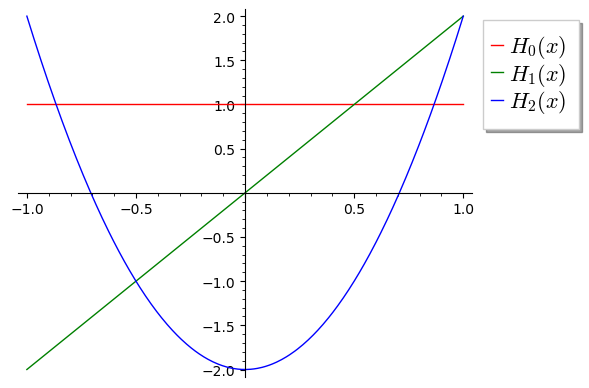
\includegraphics[width=5cm]{img/C2/Hermite1.png} & 
        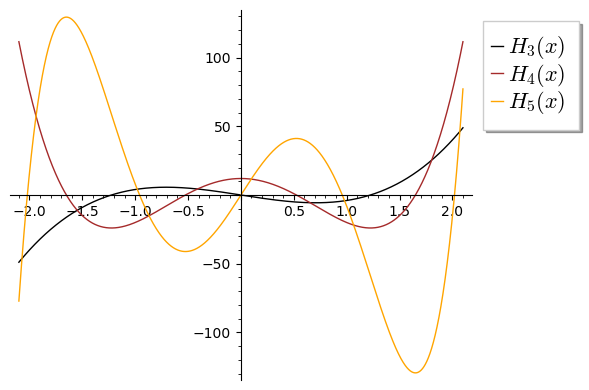
\includegraphics[width=5cm]{img/C2/Hermite2.png} &
        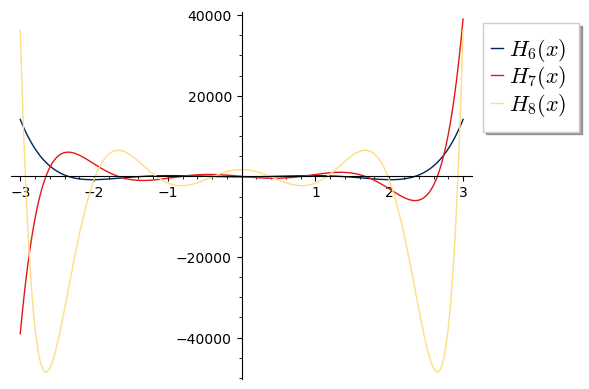
\includegraphics[width=5cm]{img/C2/Hermite3.png} \\
        (a) $H_0, H_1, H_2$ & (b) $H_3, H_4, H_5$ & (c) $H_6, H_7, H_8$ 
    \end{tabular}
    \caption{Polinomios de Hermite}
    \label{img:graficas-Hermite}
\end{figure}

La primera evidencia es que los polinomios son pares cuando el grado $n$ es par, e impares cuando el grado es impar. Por otra parte, nótese que el rango de representación del eje $X$ escogido en cada una de las tres imágenes es cada uno mayor que el anterior. Esto se debe a que se ha buscado representar todos los ceros de cada polinomio en la gráfica, y recordemos que el intervalo $[x_{n1},x_{nn}]$ es cada vez más grande conforme $n$ aumenta (véase corolario \ref{cor:sucesiones-ceros}). De hecho, si quisiéramos representar todos los ceros de todos los polinomios de Hermite sería imposible, pues el verdadero intervalo de ortogonalidad es $I=(-\infty,+\infty)$.

\subsection{Polinomios de Laguerre}

Los polinomios de Laguerre, tal y como indica su notación, $\{L^{(\alpha)}_n\}$, admiten un parámetro real $\alpha > -1$. Además, su intervalo de ortogonalidad es $[0,+\infty)$, por lo que representaremos subconjuntos acotados de este intervalo. En las imágenes \ref{img:graficas-Laguerre-alpha} podemos ver gráficas de los polinomios de Laguerre para distintos valores de $\alpha$ y un grado fijo. En particular, las imágenes \ref{img:graficas-Laguerre-alpha}(a) y \ref{img:graficas-Laguerre-alpha}(b) presentan gráficas para los polinomios de Laguerre de grado 2 y 3 respectivamente para valores de $\alpha=0,1,5,15,20,25$. El efecto que notamos es que a mayor valor de $\alpha$ la cola derecha es más suave y el crecimiento (resp. decrecimiento) hacia $+\infty$ (resp. $-\infty$) es más lento conforme crece $\alpha$. 

En la imagen  \ref{img:graficas-Laguerre-alpha}(c) presentamos de nuevo polinomios de Laguerre de grado 3 pero con valores de $\alpha$ pequeños en valor absoluto, concretamente $\alpha = -0.9, -0.5, 0, 0.5, 1$. Vemos que la conclusión es la misma que en las gráficas (a) y (b) salvo cambio de escala.

\begin{figure}[h]
    \centering
    \begin{tabular}{ccc}
        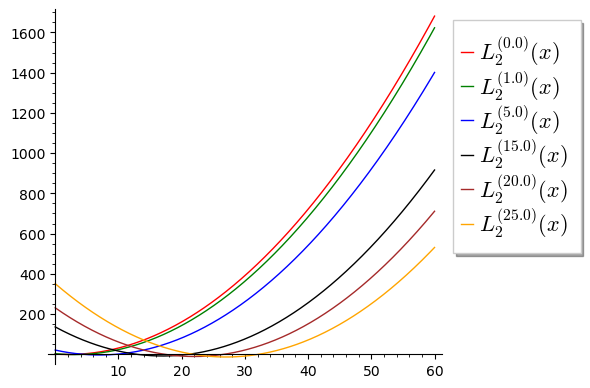
\includegraphics[width=5cm]{img/C2/Laguerre1.png} & 
        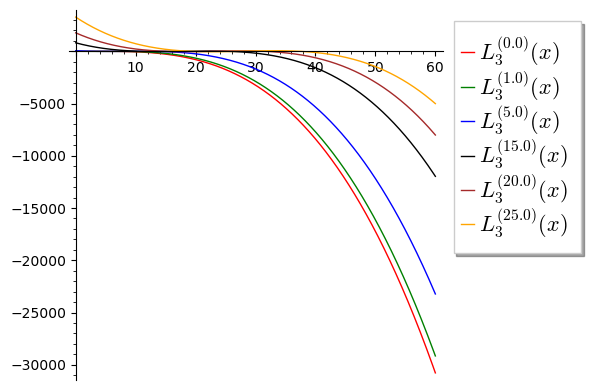
\includegraphics[width=5cm]{img/C2/Laguerre2.png} &
        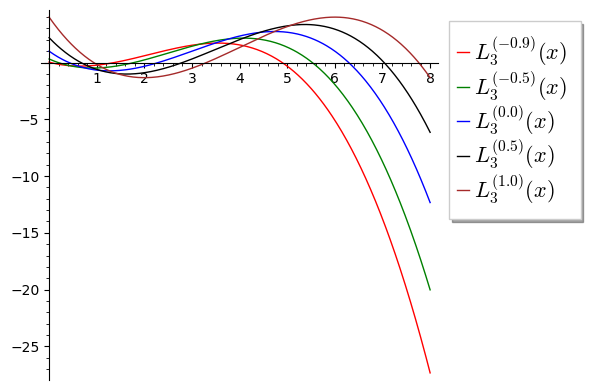
\includegraphics[width=5cm]{img/C2/Laguerre3.png} \\
        (a) Grado 2 & (b) Grado 3 & (c) Grado 3 
    \end{tabular}
    \caption{Polinomios de Laguerre con distintos valores de $\alpha$}
    \label{img:graficas-Laguerre-alpha}
\end{figure}

Véamos ahora el efecto que tiene en las gráficas el aumento del grado $n$. Para ello, fijamos $\alpha=0$ y observamos algunas imágenes en las que se ha modificado el grado. En la imagen \ref{img:graficas-Laguerre-n}(a) podemos observar las gráficas de grados 0, 1 y 2, mientras que en la imagen (b) se representan los polinomios de grados 3, 4 y 5 y en la (c) los grados 6, 7 y 8.

\begin{figure}[h]
    \centering
    \begin{tabular}{ccc}
        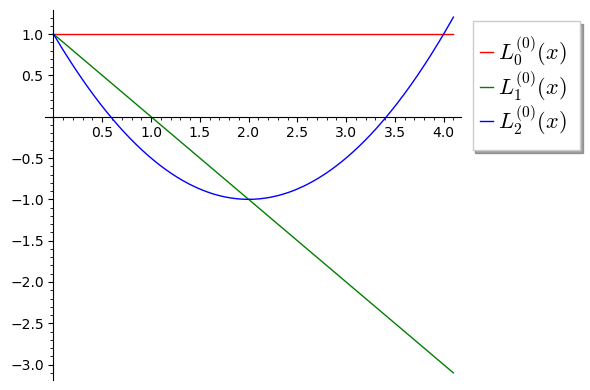
\includegraphics[width=5cm]{img/C2/Laguerre4.png} & 
        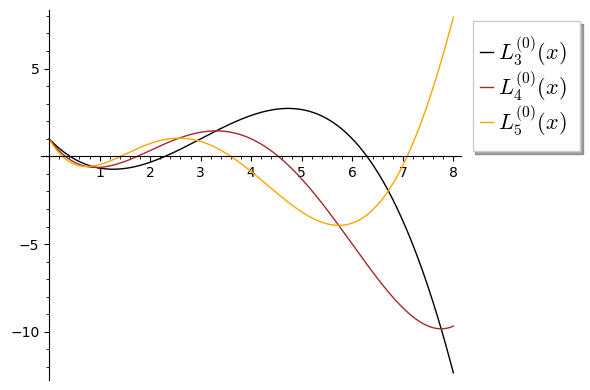
\includegraphics[width=5cm]{img/C2/Laguerre5.png} &
        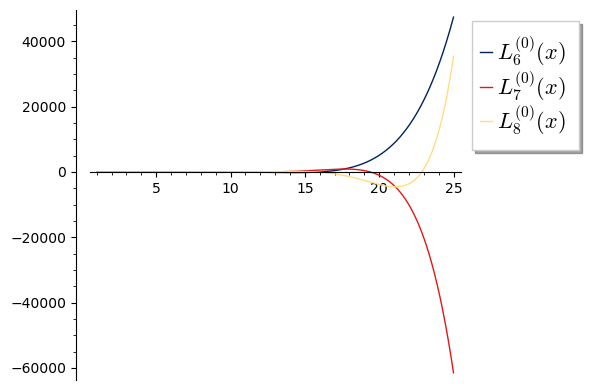
\includegraphics[width=5cm]{img/C2/Laguerre8.png} \\
        (a) $L_0^{(0)},L_1^{(0)},L_2^{(0)}$ & (b) $L_3^{(0)},L_4^{(0)},L_5^{(0)}$ & (c) $L_6^{(0)},L_7^{(0)},L_8^{(0)}$
    \end{tabular}
    \caption{Polinomios de Laguerre de distintos grados}
    \label{img:graficas-Laguerre-n}
\end{figure}

En este caso no se presenta, al menos de manera evidente, ningún tipo de simetría o paridad como sí se manifestaba en el caso de los polinomios de Hermite. Por otro lado, nótese que la gráfica (b) está truncada, es decir, no aparecen todos los ceros de todos los polinomios. Por ejemplo, aunque sabemos que $L_5^{(0)}$ tiene 5 ceros simples, únicamente representamos 4 de ellos con el objetivo de observar mejor las ondulaciones y curvas de las gráficas. Sin embargo, en la gráfica (c) sí hemos representado todos los ceros de los tres polinomios indicados, de forma que para que puedan visualizarse todos ellos en una misma gráfica se ha elegido el rango $[0,25]$ y hemos renunciado a los detalles de las curvas en valores más pequeños de $x$. 

Podemos recordar entonces la discusión sobre los ceros ya introducida en la sección anterior. Los intervalos $[x_{n1}, x_{nn}]$ son cada vez más amplios, de forma que el primer cero es cada vez más pequeño y cercano a cero, como puede verse en las imágenes \ref{img:graficas-Laguerre-n} (a) y (b), mientras que el último cero crece sin límite. Esto se debe a que el verdadero intervalo de ortogonalidad en este caso es $[0,+\infty)$.

\subsection{Polinomios de Jacobi}

Por último, analizaremos los polinomios de Jacobi $\{P_n^{(\alpha,\beta)}\}$. Estos admiten hasta dos grados de libertad $\alpha,\beta > -1$ y manifiestan su ortogonalidad en el intervalo $[-1,1]$, lo cual facilita considerablemente la representación gráfica de estos polinomios. 

\begin{figure}[h]
    \centering
    \begin{tabular}{cc}
        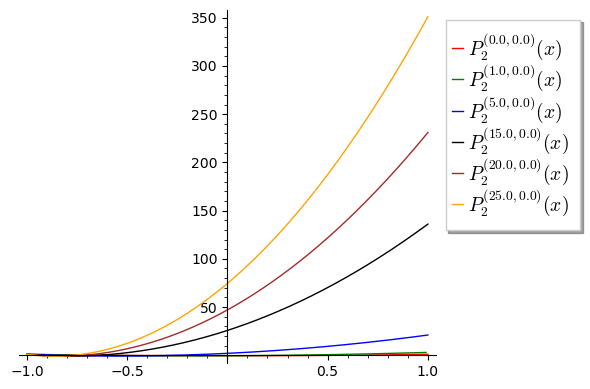
\includegraphics[width=7cm]{img/C2/Jacobi1.png} & 
        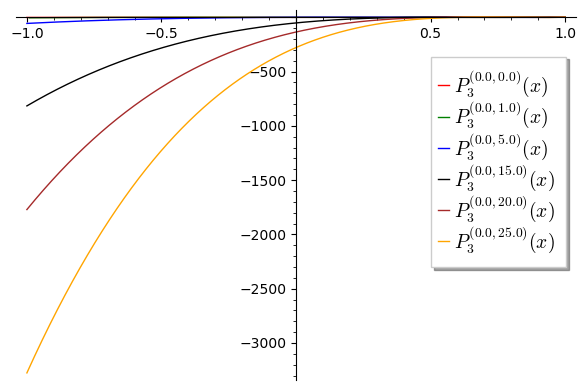
\includegraphics[width=7cm]{img/C2/Jacobi2.png} \\
        (a) Variaciones de $\alpha$ & (b) Variaciones de $\beta$ \\

        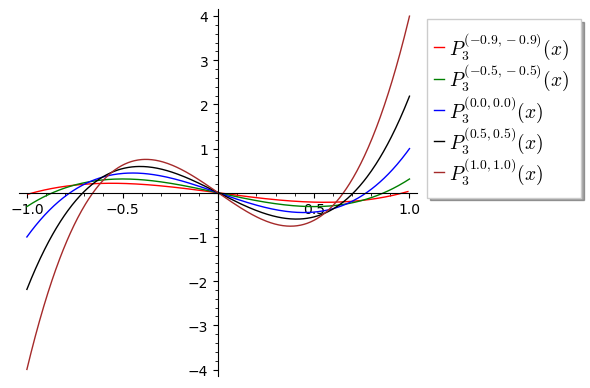
\includegraphics[width=7cm]{img/C2/Jacobi3.png} & 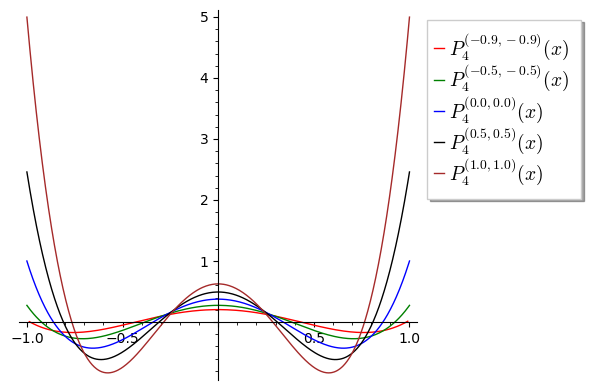
\includegraphics[width=7cm]{img/C2/Jacobi4.png} \\
        (c) Variaciones de $\alpha=\beta$ (grado 3) & (c) Variaciones de $\alpha=\beta$ (grado 4)
    \end{tabular}
    \caption{Polinomios de Jacobi con distintos valores de $\alpha$ y $\beta$}
    \label{img:graficas-Jacobi-alpha-beta}
\end{figure}

Comenzaremos analizando el efecto del parámetro $\alpha$. Para ello, hemos fijado $n=2$ y $\beta=0$, representando el polinomio de Jacobi $P_2^{(\alpha,0)}$ para los valores $\alpha=0,1,5,15,20,25$, véase la imagen \ref{img:graficas-Jacobi-alpha-beta}(a). Obsérvese que, de forma similar a los polinomios de Laguerre, este parámetro interviene en la velocidad a la que aumenta la cola derecha. Sin embargo, lo hace de forma inversa, ya que mientras que a mayores valores de $\alpha$ la inclinación era menor en los polinomios de Laguerre, en este caso conforme crece $\alpha$ aumenta también la misma.

Respecto a $\beta$, para analizar su impacto en las gráficas fijamos $n=3$ y $\alpha=0$, presentando los polinomios $P_3^{(0,\beta)}$ para $\beta=0,1,5,15,20,25$ en la imagen \ref{img:graficas-Jacobi-alpha-beta}(b). El comportamiento de $\beta$ es análogo al de $\alpha$ pero en la cola izquierda en lugar de la derecha. Es decir, a mayor valor de $\beta$, mayor inclinación de la cola derecha, que en estas gráficas se traduce en un descenso a $-\infty$ más pronunciado.

En los casos de Hermite y Laguerre hemos discutido también la paridad y/o simetría de los gráficos. A juzgar por las imágenes \ref{img:graficas-Jacobi-alpha-beta}(a) y \ref{img:graficas-Jacobi-alpha-beta}(b), los polinomios de Jacobi no cumplen ningún tipo de simetría en general. Sin embargo, en la imagen \ref{img:graficas-Jacobi-alpha-beta}(c) puede comprobarse qué ocurre al igualar $\alpha=\beta$. En efecto, en este caso las gráficas son simétricas respecto al eje $Y$ cuando el grado es par ($P_{2n}^{(\alpha,\alpha)}$ es par). Respectivamente, $P_{2n+1}^{(\alpha,\alpha)}$ es impar. 

Finalmente, comprobemos gracias a las imágenes \ref{img:graficas-Jacobi-n} la variación de estas gráficas al aumentar el grado cuando fijamos $\alpha = \beta = 0$.

\begin{figure}[h]
    \centering
    \begin{tabular}{ccc}
        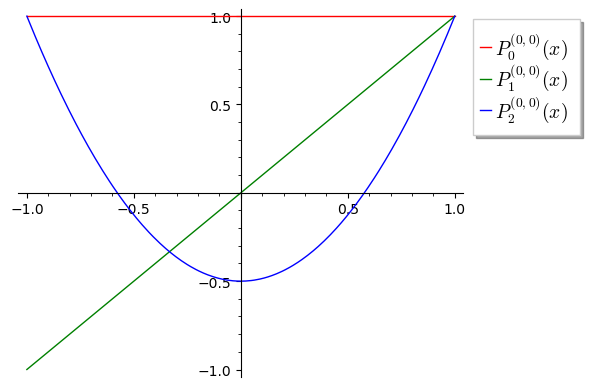
\includegraphics[width=5cm]{img/C2/Jacobi5.png} & 
        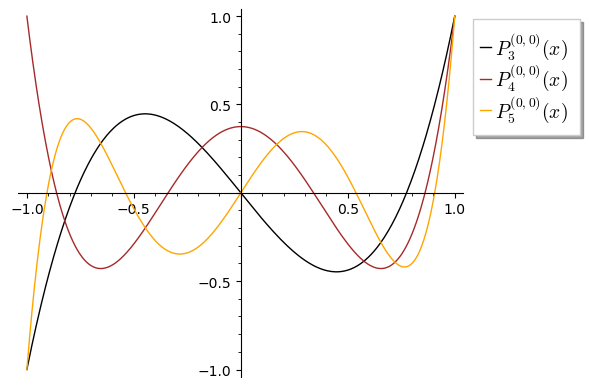
\includegraphics[width=5cm]{img/C2/Jacobi6.png} &
        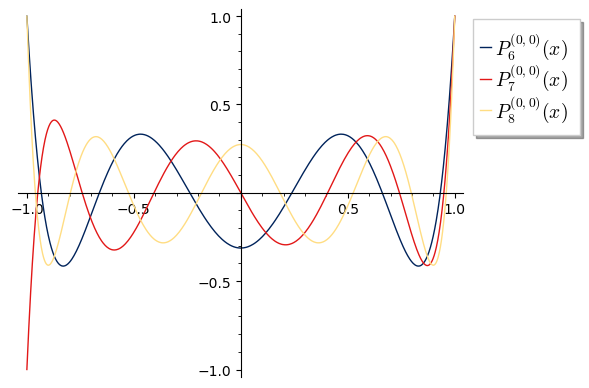
\includegraphics[width=5cm]{img/C2/Jacobi7.png} \\
        (a) $P_0^{(0,0)},P_1^{(0,0)},P_2^{(0,0)}$ & (b) $P_3^{(0,0)},P_4^{(0,0)},P_5^{(0,0)}$ & (c) $P_6^{(0,0)},P_7^{(0,0)},P_8^{(0,0)}$
    \end{tabular}
    \caption{Polinomios de Jacobi de distintos grados}
    \label{img:graficas-Jacobi-n}
\end{figure}

En estas tres figuras se puede comprobar más fácilmente la paridad e imparidad de los polinomios de Jacobi en el caso $\alpha=\beta$ con respecto al grado $n$. Como además el intervalo de ortogonalidad es $I=[-1,1]$, todos los ceros de estos polinomios están representados siempre en el mismo.